
\documentclass[fleqn,addpoints]{exam}

\usepackage{graphicx}
\usepackage{float}
\usepackage{amsmath}
\usepackage{cancel}
\usepackage{polynom}
\usepackage{caption}

\printanswers

\ifprintanswers 
\usepackage{2in1, lscape} 
\fi

\title{Math 115 \\ Homework 17}
\date{\today}

\begin{document}

\maketitle

% \begin{figure}[H]
%   \centering
%   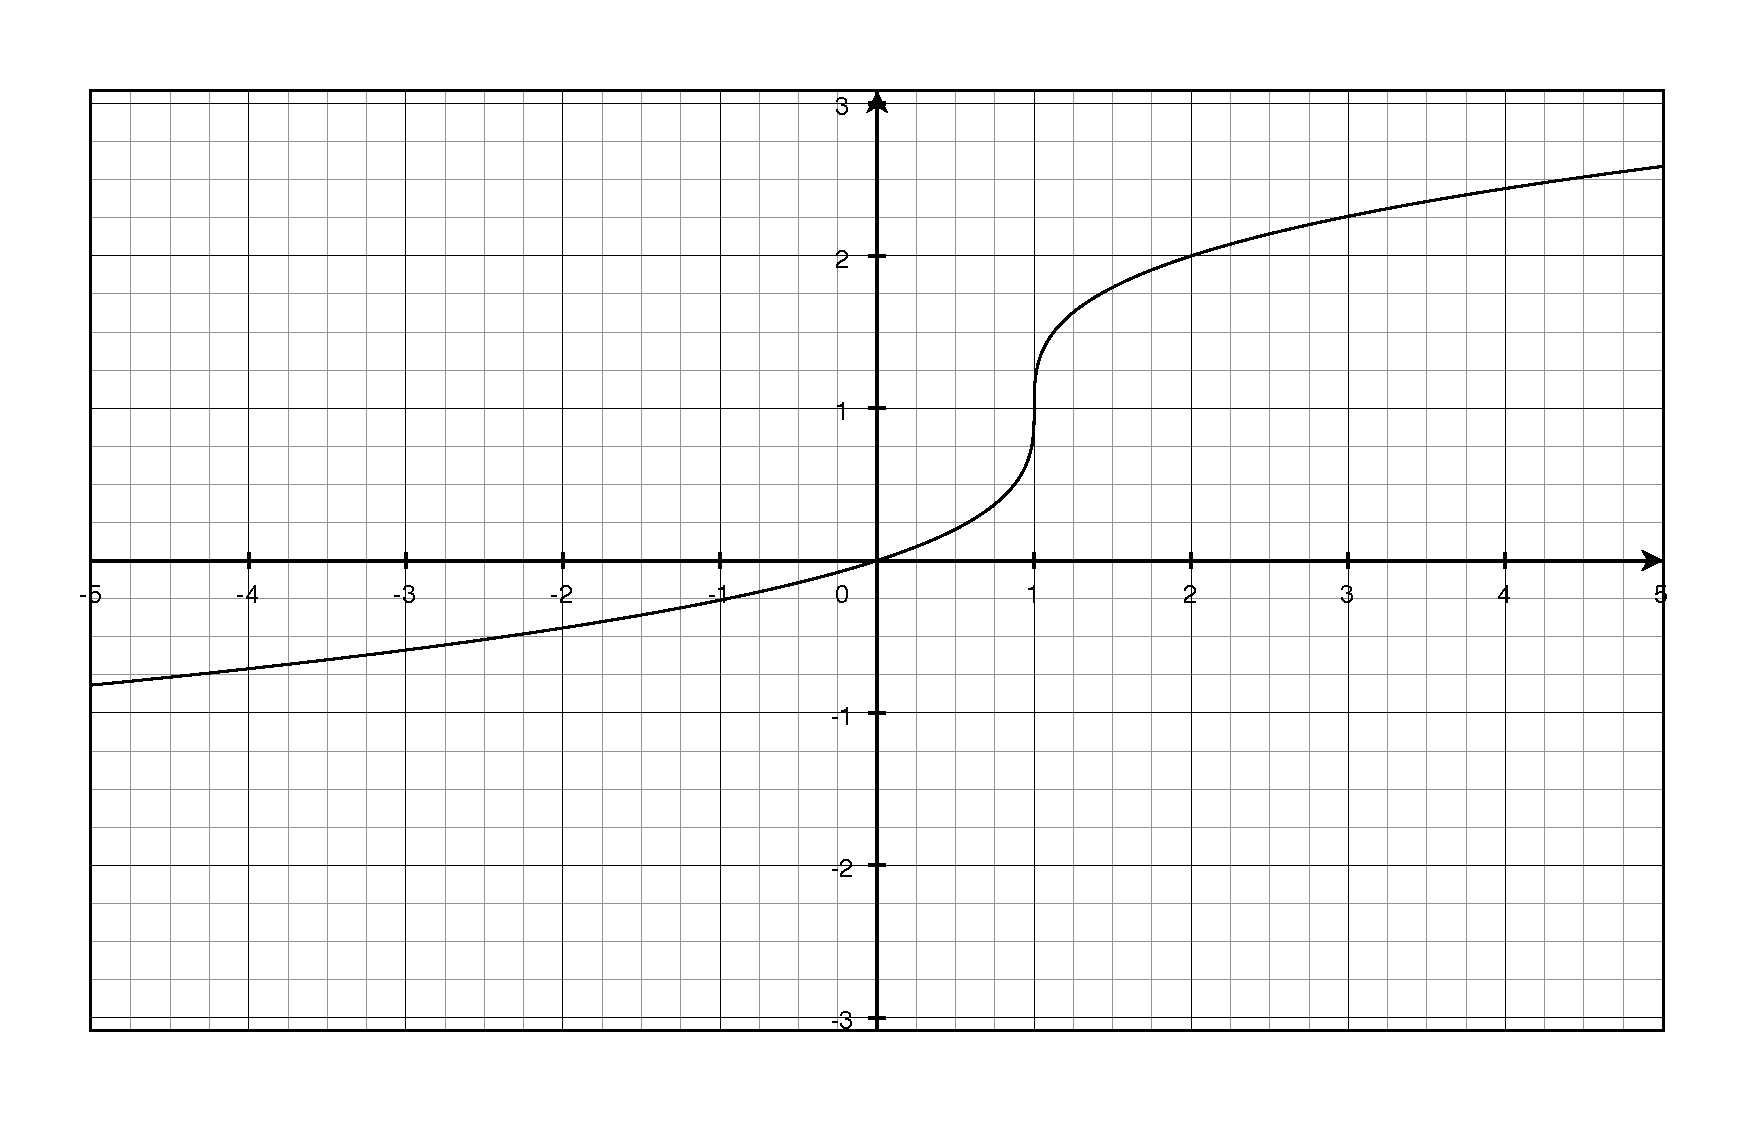
\includegraphics[scale=.3]{question7.eps}
%   \caption*{Question 7}
% \end{figure}

\section{Homework}

\begin{itemize}
  \item Read Section 3.4
  \item pp 324-327: 11-15, 24-25, 28-30, 35-39, 45-49, 60-64, 80-81, 90-91, 95-96, 100-101, 111, 115, 118
\end{itemize}

For the questions which ask you to approximate to 3 decimal places, you can just leave the answer as $e^2$ (or whatever
it is) if you don't have a calculator.

\section{Extra Credit}

p. 327, question 127

\ifprintanswers

\section{Section 3.4}

\begin{description}

\item[11]
\begin{align*}
  7^x &= \frac{1}{49} \\
  \log_7 7^x &= \log_7 \frac{1}{49} \\
  \log_7 7^x &= \log_7 7^{-2} \\
  x &= -2 \\
\end{align*}

\item[12]
\begin{align*}
  8^x &= 4 \\
  \log_8 8^x &= \log_8 4 \\
  x &= \frac{2}{3} \\
\end{align*}

\item[13]
\begin{align*}
  \left( \frac{1}{2} \right)^x &= 32 \\
  \log_{\frac{1}{2}} \left( \frac{1}{2} \right)^x &= \log_{\frac{1}{2}} 32 \\    
  x &= -5 \\
\end{align*}

\item[14]
\begin{align*}
  \left( \frac{1}{4} \right)^x &= 64 \\
  \log_{\frac{1}{4}} \left( \frac{1}{4} \right)^x &= \log_{\frac{1}{4}} 64 \\
  x &= -3 \\
\end{align*}

\item[15]
\begin{align*}
  \left( \frac{3}{4} \right) ^x &= \frac{27}{64} \\
  \log_{\frac{3}{4}} \left( \frac{3}{4} \right) ^x &= \log_{\frac{3}{4}} \frac{27}{64} \\
  x &= 3 \\
\end{align*}

\item[24]
\begin{align*}
  \ln x &= -7 \\
  e^{\ln x} &= e^{-7} \\
  x &= e^{-7} \\
\end{align*}

\item[25]
\begin{align*}
  \log_4 x &= 3 \\
  4^{\log_4 x} &= 4^3 \\
  x &= 64 \\
\end{align*}

\item[28]
\begin{align*}
  \log_{10} x + 3 &= 0 \\
  \log_{10} x &= -3 \\
  10^{\log_{10} x} &= 10^{-3} \\
  x &= \frac{1}{1000} \\
\end{align*}

\item[29]
\begin{align*}
  \log_{10} x &= -1 \\
  10^{\log_{10} x} &= 10^{-1} \\
  x &= \frac{1}{10} \\
\end{align*}

\item[30]
\begin{align*}
  \ln (2x - 1) &= 0 \\
  e^{\ln(2x - 1)} &= e^0 \\
  2x - 1 &= 1 \\
  2x  &= 2 \\
  x  &= 1 \\
\end{align*}

\item[35]
\[
  \log_{10} 10^{x^2} = x^2
\]

\item[36]
\[
  \log_{6} 6^{2x-1} = 2x-1
\]

\item[37]
\[
  8^{\log_8 (x-2)} = x-2
\]

\item[38]
\[
  4^{\log_4 x^3} = x^3
\]

\item[39]
\[
  \ln e^{7x+2} = 7x+2
\]

\item[45]
\begin{align*}
  e^x &= 10 \\
  x &= \ln 10 \\
  x &\approx 2.303 \\
\end{align*}

\item[46]
\begin{align*}
  4 e^x &= 91 \\
  e^x &= 22.75 \\
  x &= \ln 22.75 \\  
  x &\approx 3.125 \\
\end{align*}

\item[47]
\begin{align*}
  7 - 2e^x &= 5 \\
   2e^x &= 2 \\
   e^x &= 1 \\
   x &= 0 \\
\end{align*}

\item[48]
\begin{align*}
  -14 + 3e^x &= 11 \\
  3e^x &= 25 \\
  e^x &= \frac{25}{3} \\
  x &= \ln \frac{25}{3} \\
  x &\approx 2.120
\end{align*}

\item[49]
\begin{align*}
  e^{3x} &= 12 \\
  3x &= \ln 12 \\
  x &= \frac{\ln 12}{3} \\
  x &\approx 0.828 \\
\end{align*}

\item[60]
\begin{align*}
  6^{5x} &= 3000 \\
  5x &= \log_6 3000 \\
  5x &= \frac{\ln 3000}{\ln 6} \\
  x &= \frac{\ln 3000}{5 \ln 6} \\
  x &\approx 0.894 \\
\end{align*}

\item[61]
\begin{align*}
  5^{-t/2} &= 0.20 \\
  -\frac{t}{2} &= \log_5 0.20 \\
  -\frac{t}{2} &= \log_5 5^{-1} \\
  -\frac{t}{2} &= -1 \\
  t &= 2 \\
\end{align*}

\item[62]
\begin{align*}
  4^{-3t} &= 0.10 \\
  -3t &= \log_4 1/10 \\
  -3t &= \log_4 10^{-1} \\
  -3t &= -\log_4 10 \\
  3t &= \log_4 10 \\
  3t &= \frac{\log_{10} 10}{\log_{10} 4} \\
  3t &= \frac{1}{\log_{10} 4} \\
  t &= \frac{1}{3 \log_{10} 4} \\
  t &\approx 0.554 \\
\end{align*}

\item[63]
\begin{align*}
  2^{3-x} &= 565 \\
  3-x &= \log_2 565 \\
  -x &= \log_2 565 - 3\\
  x &= 3 - \log_2 565 \\
  x &= 3 - \frac{\ln 565}{\ln 2} \\
  x &\approx -6.142 \\
\end{align*}

\item[64]
\begin{align*}
  8^{-2-x} &= 431 \\
  -2-x &= \log_8 431 \\
  -x &= \log_8 431 + 2 \\
  x &= - \log_8 431 - 2 \\
  x &= - \frac{\ln 431}{\ln 8} - 2 \\
  x &\approx -4.917 \\
\end{align*}

\item[80]
\begin{align*}
  \left(16 - \frac{0.878}{26} \right)^{3t} &= 30 \\
  15.966^{3t} &= 30 \\
  3t &= \log_{15.966} 30 \\
  3t &= \frac{\ln 30}{\ln 15.966} \\
  t &= \frac{\ln 30}{3 \ln 15.966} \\
  t &\approx 0.409
\end{align*}

\item[81]
\begin{align*}
  \frac{3000}{2 + e^{2x}} &= 2 \\
  3000 &= 4 + 2e^{2x} \\
  2e^{2x} &= 2996 \\
  e^{2x} &= 1498 \\
  2x &= \ln 1498 \\
  x &= \frac{\ln 1498}{2} \\
  x &\approx 3.656 \\
\end{align*}

\item[90]
\begin{align*}
  \ln \sqrt{x-8} &= 5 \\
  \ln (x-8)^{1/2} &= 5 \\
  \frac{1}{2} \ln (x-8) &= 5 \\
  \ln (x-8) &= 10 \\
  x-8 &= e^{10} \\
  x &= e^{10} + 8\\
  x &\approx 22034.466
\end{align*}

\item[91]
\begin{align*}
  \ln (x+1)^2 &= 2 \\
  2 \ln (x+1) &= 2 \\
  \ln (x+1) &= 1 \\
  x+1 &= e \\
  x &= e - 1\\
  x &\approx 1.718
\end{align*}

\item[95]
\begin{align*}
  \ln(x+5) &= \ln(x-1) - \ln(x+1) \\
  \ln(x+5) &= \ln \left( \frac{x-1}{x+1} \right) \\
  x+5 &= \frac{x-1}{x+1} \\
  x^2 + 6x + 5 &= x-1 \\
  x^2 + 5x + 6 &= 0 \\
  (x+2)(x+3) &= 0 \\
  x &= \{-2, -3\}
\end{align*}

Neither of the two possible solutions is in the domain, so there is no solution.

\item[96]
\begin{align*}
  \ln(x+1) - \ln(x-2) &= \ln x^2 \\
  \ln \left( \frac{x+1}{x-2} \right) &= \ln x^2 \\
  \frac{x+1}{x-2} &= x^2 \\
  x+1 = x^2(x-2) \\
  x+1 = x^3-2x^2 \\
  x^3 -2x^2 - x - 1 &= 0 \\
\end{align*}

$x \approx 2.5468$ using a graphing calculator.  I don't know how else you would find the solution, so I should have done this
problem before including it in the homework. 

\item[100]
\begin{align*}
  5 \log(x-2) &= 11 \\
  \log(x-2) &= \frac{11}{5} \\
  x-2 &= 10^{11/5} \\
  x &= 10^{11/5} + 2 \\
  x &\approx 160.489 \\
\end{align*}

\item[101]
\begin{align*}
  \log(x+4) - \log x &= \log(x+2) \\
  \log \left( \frac{x+4}{x} \right) &= \log(x+2) \\
  \frac{x+4}{x} &= x+2 \\
   x^2 + x - 4 &= 0 \\
   x &= \frac{-1 \pm \sqrt{17}}{2} \\
   x &\approx \{ -2.562, 1.562 \}
\end{align*}

$-2.562$ isn't in the domain so 1.562 is the only solution.

\item[111]
\begin{align*}
  2A_0 &= A_0 e^{rt} \\
  2 &= e^{rt} \\
  t &= \frac{\ln 2}{r} \\
\end{align*}

For $r = 0.085$, $t \approx 8.155$ years.  The amount doesn't matter since the same time works for any amount.

\item[115]
\begin{align*}
  p &= 500 - 0.5 e^{0.004x} \\
  p - 500 &= -0.5 e^{0.004x} \\
  e^{0.004x} &= \frac{500 - p}{0.5} \\
  e^{0.004x} &= 1000 - 2p \\
  0.004x &= \ln(1000 - 2p) \\
  x &= \frac{\ln(1000 - 2p)}{0.004} \\
\end{align*}

\begin{description}
\item[a]
For $p = 350$, $x \approx 1426$

\item[b]
For $p = 300$, $x \approx 1498$
\end{description}

\item[118]
\begin{align*}
  21 &= 68 \cdot 10^{-0.04x} \\
  \frac{21}{68} &= 10^{-0.04x} \\
  \log \left( \frac{21}{68} \right) &= -0.04x \\
  x &\approx 12.758 \\
\end{align*}

\end{description}


\else

\vspace{4 in}

{\em If I were asked to answer the following question: What is slavery? and I should answer in one word, It is murder!,
  my meaning would be understood at once. No extended argument would be required . . . Why, then, to this other
  question: What is property? may I not likewise answer, It is robbery!, without the certainty of being misunderstood;
  the second proposition being no other than a transformation of the first?}

\vspace{.1 cm}
\hspace{1 cm} --Pierre-Joseph Proudhon
\fi
\end{document}

